% !TEX root = ./report.tex

\subsection{Input file}

Now let's have a look at the input file.
A typical input file has structure like:
\begin{verbatim}
Test                              (title)
md                                (calc)
s       n                         (ic,iio)
10.00000                          (alatt)
1       1       1                 (nsc)
1.00000   0.00000   0.00000       (avec)
0.00000   1.00000   0.00000
0.00000   0.00000   1.00000
0.00100   0.00000                 (cmass, press)
1                                 (ntype)
4       Ar      36.00000          (natom,nameat,atmass)
0.00000   0.00000   0.00000       (rat)
0.50000   0.50000   0.00000
0.00000   0.50000   0.50000
0.50000   0.00000   0.50000
40                                (rcut)
6       6       6                 (ncell)
1000    100     10                (nstep,ntcheck,ntimes)
0.00000   0.00100   200.00000     (temp,ttol,dt)
\end{verbatim}

This input file investigates $4$ \ce{Ar} atoms in a FCC cell, the atom mass is assumed to be \SI{36.0}{\atomicmassunit},
see Fig. \ref{fig:fcc1} for the structure of this cell.
The \texttt{calc} specifies calculation type of this file, including \texttt{md},
\texttt{cd}, \texttt{nd}, \texttt{sd}, as we mentioned in the beginning of Sec. \ref{sec:mdc}.
\texttt{nsc} means the number of cells consist a supercell in each direction of a 3D space.
\texttt{cmass} is $W$ as mentioned, but it does not have functions for \texttt{md}.
\texttt{rcut} is the cut-off radius for this molecular dynamics, and the sphere defined by
\texttt{rcut} must be contained inside the stack of supercells, which is $7=2\times 3+1$ supercells in each direction. We usually choose numbers for \texttt{ncell}, to make
\texttt{alatt} times \texttt{ncell} greatly larger than \texttt{rcut}, for the supercells are
oscillating their volume in this molecular dynamics.
Here we have $4=4 \times 1^3$ atoms inside one supercell.
Make sure that \texttt{ntcheck} times \texttt{ntimes} is greater than
\texttt{nstep}.
And \texttt{dt} times \texttt{nstep} is the total simulation time in Rydberg unit, which is
\SI{4.8378e-17}{\second} per unit time.

\begin{figure}[H]
\begin{minipage}{0.48\textwidth}
	\centering
	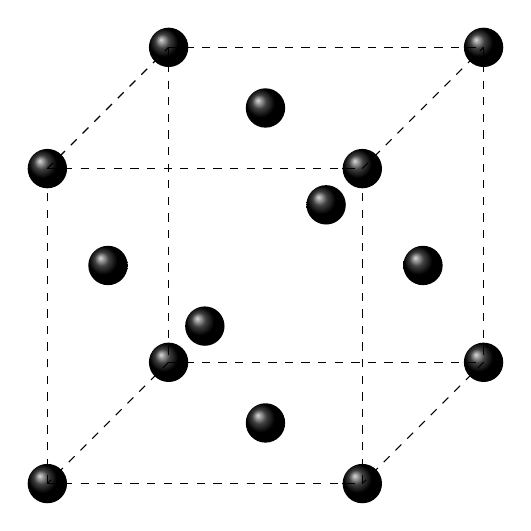
\begin{tikzpicture}
 %points on cube
 \coordinate (A) at (0,0,0);
 \coordinate (B) at (0,0,4);
 \coordinate (D) at (0,4,0);
 \coordinate (C) at (0,4,4);
 \coordinate (E) at (4,0,0);
 \coordinate (F) at (4,0,4);
 \coordinate (H) at (4,4,0);
 \coordinate (G) at (4,4,4);

 %center of faces
 \coordinate (I) at (0,2,2); %center of face ABCD
 \coordinate (J) at (4,2,2); %center of face EFGH
 \coordinate (K) at (2,4,2); %center of face DCGH
 \coordinate (L) at (2,0,2); %center of face ABFE
 \coordinate (M) at (2,2,4); %center of face CBGF
 \coordinate (N) at (2,2,0); %center of face DAEH

 %place non-atom cube corners
 \shade [ball color= black] (A) circle (0.25cm);
 \shade [ball color= black] (C) circle (0.25cm);
 \shade [ball color= black] (F) circle (0.25cm);
 \shade [ball color= black] (H) circle (0.25cm);
 \shade [ball color= black] (B) circle (0.25cm);
 \shade [ball color= black] (D) circle (0.25cm);
 \shade [ball color= black] (E) circle (0.25cm);
 \shade [ball color= black] (G) circle (0.25cm);

 %draw the center of each face
 \shade [ball color= black] (I) circle (0.25cm);
 \shade [ball color= black] (J) circle (0.25cm);
 \shade [ball color= black] (K) circle (0.25cm);
 \shade [ball color= black] (L) circle (0.25cm);
 \shade [ball color= black] (M) circle (0.25cm);
 \shade [ball color= black] (N) circle (0.25cm);

 %draw cube
 \draw [dashed] (A) -- (B);
 \draw [dashed] (B) -- (C);
 \draw [dashed] (C) -- (D);
 \draw [dashed] (D) -- (A);
 \draw [dashed] (E) -- (F);
 \draw [dashed] (F) -- (G);
 \draw [dashed] (G) -- (H);
 \draw [dashed] (H) -- (E);
 \draw [dashed] (A) -- (E);
 \draw [dashed] (B) -- (F);
 \draw [dashed] (C) -- (G);
 \draw [dashed] (D) -- (H);
\end{tikzpicture}

	\caption{A FCC conventional unit cell of \ce{Ar} for \texttt{inp1}.}
	\label{fig:fcc1}
\end{minipage}
\hfill
\begin {minipage}{0.48\textwidth}
\centering
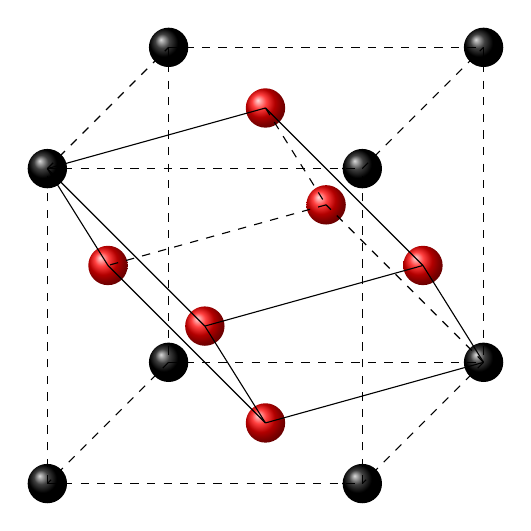
\begin{tikzpicture}
 %points on cube
 \coordinate (A) at (0,0,0);
 \coordinate (B) at (0,0,4);
 \coordinate (D) at (0,4,0);
 \coordinate (C) at (0,4,4);
 \coordinate (E) at (4,0,0);
 \coordinate (F) at (4,0,4);
 \coordinate (H) at (4,4,0);
 \coordinate (G) at (4,4,4);

 %center of faces
 \coordinate (I) at (0,2,2); %center of face ABCD
 \coordinate (J) at (4,2,2); %center of face EFGH
 \coordinate (K) at (2,4,2); %center of face DCGH
 \coordinate (L) at (2,0,2); %center of face ABFE
 \coordinate (M) at (2,2,4); %center of face CBGF
 \coordinate (N) at (2,2,0); %center of face DAEH

 %place non-atom cube corners
 \shade [ball color= black] (A) circle (0.25cm);
 \shade [ball color= black] (C) circle (0.25cm);
 \shade [ball color= black] (F) circle (0.25cm);
 \shade [ball color= black] (H) circle (0.25cm);
 \shade [ball color= black] (B) circle (0.25cm);
 \shade [ball color= black] (D) circle (0.25cm);
 \shade [ball color= black] (E) circle (0.25cm);
 \shade [ball color= black] (G) circle (0.25cm);

 %draw the center of each face
 \shade [ball color= red] (I) circle (0.25cm);
 \shade [ball color= red] (J) circle (0.25cm);
 \shade [ball color= red] (K) circle (0.25cm);
 \shade [ball color= red] (L) circle (0.25cm);
 \shade [ball color= red] (M) circle (0.25cm);
 \shade [ball color= red] (N) circle (0.25cm);

 %draw cube
 \draw [dashed] (A) -- (B);
 \draw [dashed] (B) -- (C);
 \draw [dashed] (C) -- (D);
 \draw [dashed] (D) -- (A);
 \draw [dashed] (E) -- (F);
 \draw [dashed] (F) -- (G);
 \draw [dashed] (G) -- (H);
 \draw [dashed] (H) -- (E);
 \draw [dashed] (A) -- (E);
 \draw [dashed] (B) -- (F);
 \draw [dashed] (C) -- (G);
 \draw [dashed] (D) -- (H);
 
 %draw unit cell
 \draw (E) -- (L);
 \draw (E) -- (J);
 \draw [dashed] (E) -- (N);
 \draw (J) -- (M);
 \draw (L) -- (M);
 \draw (J) -- (K);
 \draw [dashed] (K) -- (N);
 \draw (K) -- (C);
 \draw (M) -- (C);
 \draw (L) -- (I);
 \draw [dashed] (N) -- (I);
 \draw (C) -- (I);
\end{tikzpicture}

\caption{A FCC primitive unit cell of \ce{Ar} for \texttt{inp3}, with
	vertices of the cell filled in red.}
\label{fig:fcc3}
\end{minipage}
\end{figure}

Now we are going to play with Wentzcovitch's molecular dynamics, to see what the
actual ``dynamics'' it is. Suppose we have such a file as \texttt{inp1}:
\begin{verbatim}
Test                              (title)
nd                                (calc)
s       n                         (ic,iio)
11.00000                          (alatt)
1       1       1                 (nsc)
1.00000   0.00000   0.00000       (avec)
0.00000   1.00000   0.00000
0.00000   0.00000   1.00000
0.00100   0.00000                 (cmass, press)
1                                 (ntype)
4       Ar      36.00000          (natom,nameat,atmass)
0.00000   0.00000   0.00000       (rat)
0.50000   0.50000   0.00000
0.00000   0.50000   0.50000
0.50000   0.00000   0.50000
40                                (rcut)
6       6       6                 (ncell)
2000    100     10                (nstep,ntcheck,ntimes)
0.00000   0.00100   75.00000      (temp,ttol,dt)
\end{verbatim}
We will use this file as an example for comparison.
The \texttt{press} is external pressure $P$, but in unit of \si{\mega\bar}.

Here we are going to use $h = 75$ Rydberg unit and $2000$ time steps. This is because, different \texttt{dt} could result in different decaying rates.
We run this file with $4$ different \texttt{dt}, $150$, $200$, $300$ and $400$
Rydberg unit respectively.
But we simulate both $600000$ Rydberg time unit. From Fig. \ref{fig:inp1:mini:subfig:b} we can see a noticeable
decreasing in total energy, but for Fig. \ref{fig:inp1:mini:subfig:a} this is less distinguishable. For Fig. \ref{fig:inp1:mini:subfig:c} and Fig. \ref{fig:inp1:mini:subfig:d}
this is even worse, the total energy decays even faster. This can be understood since in
Beeman's algorithm we assume the length of each time step $h$ is a small quantity,
for we are using Taylor expansion implicitly. So when $h$ is too large, numerical errors
could be apparent.

\begin{figure}[h]
	\centering
	\subfigure[$4000$ time steps, with each time step to be $150$ Rydberg unit.]{
		\label{fig:inp1:mini:subfig:a}   %% label for second subfigure 
		\begin{minipage}[b]{0.48\textwidth}
			\centering
			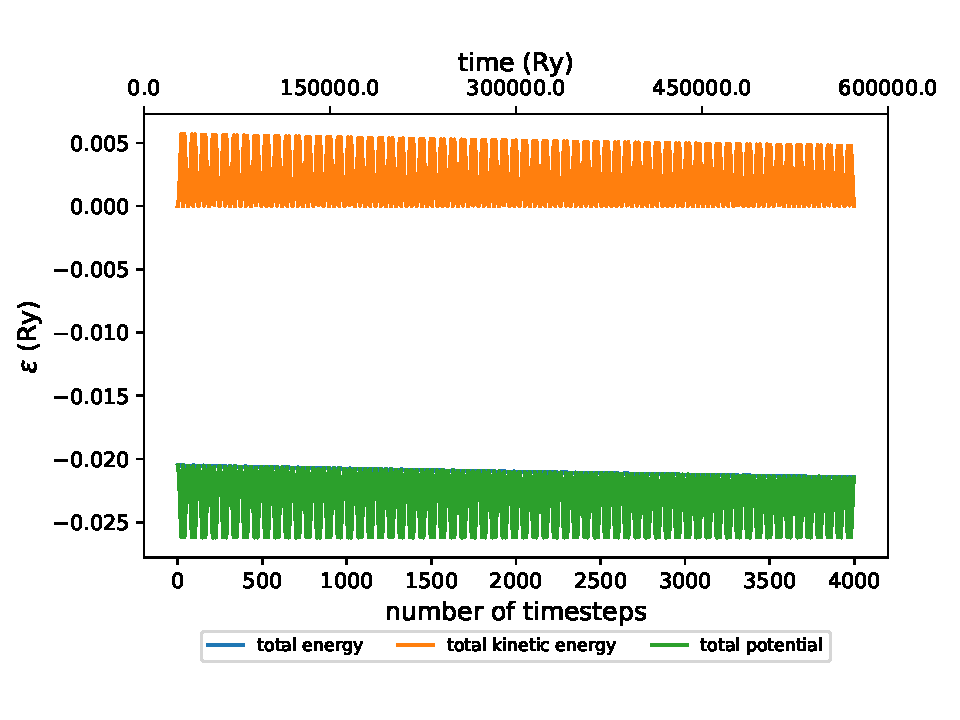
\includegraphics[width=\linewidth]{4000_150_100_4}
		\end{minipage}}
	\hfill
	\subfigure[$3000$ time steps, with each time step to be $200$ Rydberg unit.]{
		\label{fig:inp1:mini:subfig:b}   %% label for first subfigure 
		\begin{minipage}[b]{0.48\textwidth}
			\centering
			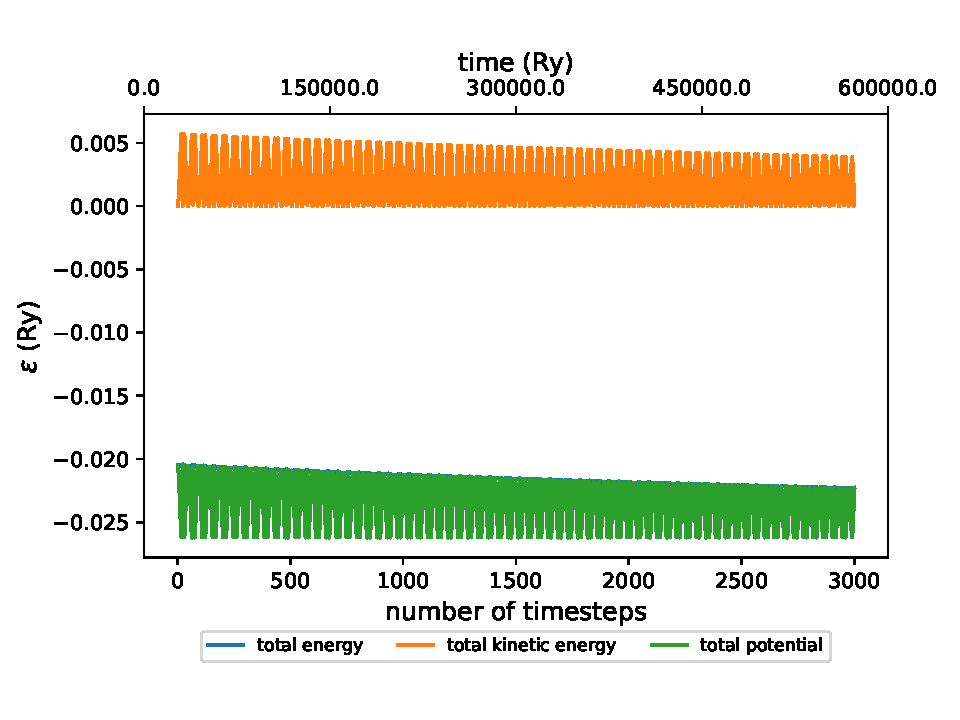
\includegraphics[width=\linewidth]{3000_200_100_9}
		\end{minipage}}
	\subfigure[$2000$ time steps, with each time step to be $300$ Rydberg unit.]{
		\label{fig:inp1:mini:subfig:c}   %% label for third subfigure 
		\begin{minipage}[b]{0.48\textwidth}
			\centering
			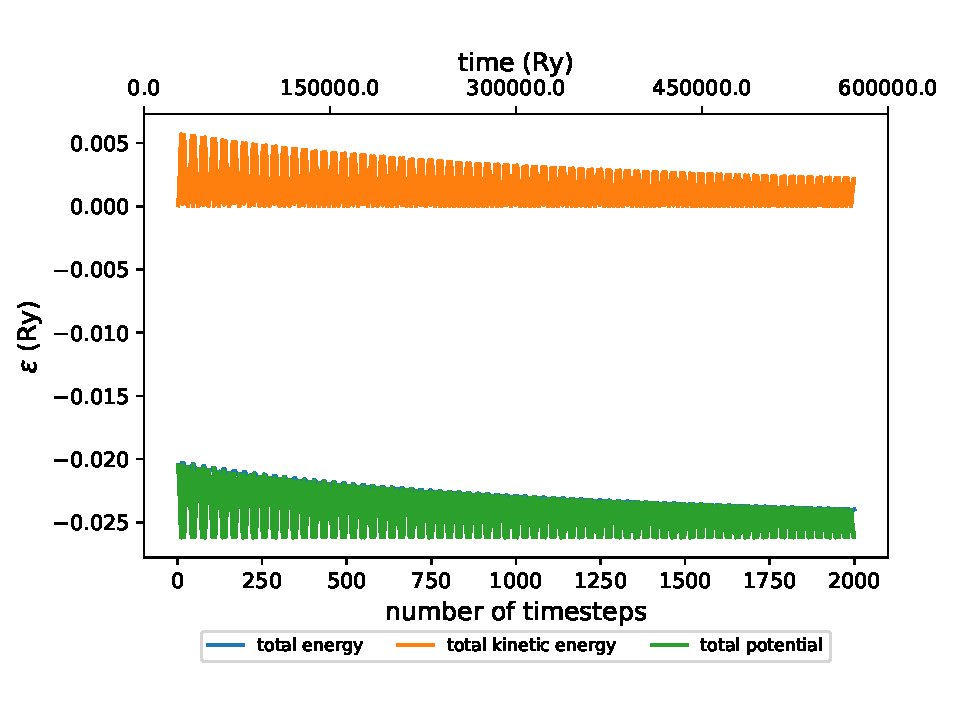
\includegraphics[width=\linewidth]{2000_300_100_0}
		\end{minipage}}
	\hfill
	\subfigure[$1500$ time steps, with each time step to be $400$ Rydberg unit.]{
		\label{fig:inp1:mini:subfig:d}   %% label for fourth subfigure 
		\begin{minipage}[b]{0.48\textwidth}
			\centering
			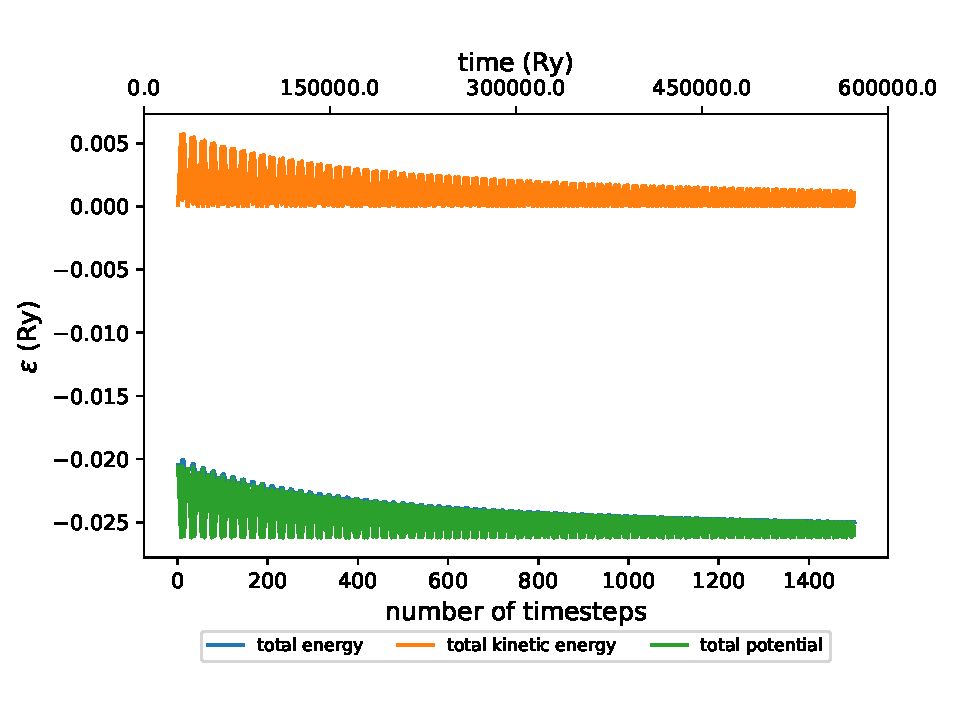
\includegraphics[width=\linewidth]{1500_400_100_2}
		\end{minipage}}
	\caption{Wentzcovitch MD for FCC \ce{Ar} at \SI{0}{\kelvin} with $4$ different \texttt{dt} but the same total simulation time.}
	\label{fig:inp1}   %% label for entire figure 
\end{figure}

So for easier observation $h = 75$ Rydberg unit and $2000$ time steps are good choices,
see Fig. \ref{fig:inp1run} for references.

\begin{figure}[h]
	\subfigure[Energies of the cell and atoms versus time.]{
		\label{fig:inp1run:mini:subfig:a}   %% label for first subfigure 
		\begin{minipage}[b]{0.48\textwidth}
			\centering
			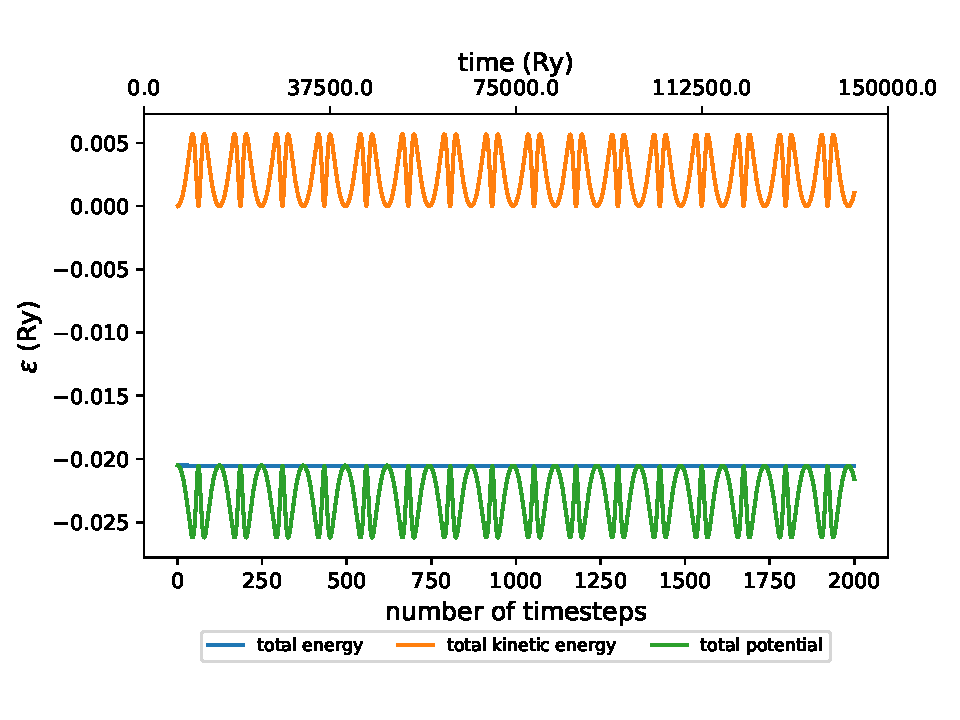
\includegraphics[width=\linewidth]{2000_75_100_8}
		\end{minipage}}
	\hfill
	\subfigure[Cell vectors oscillation versus time, $a=b=c$ for this is a cubic crystal.]{
		\label{fig:inp1run:mini:subfig:b}   %% label for second subfigure 
		\begin{minipage}[b]{0.48\textwidth}
			\centering
			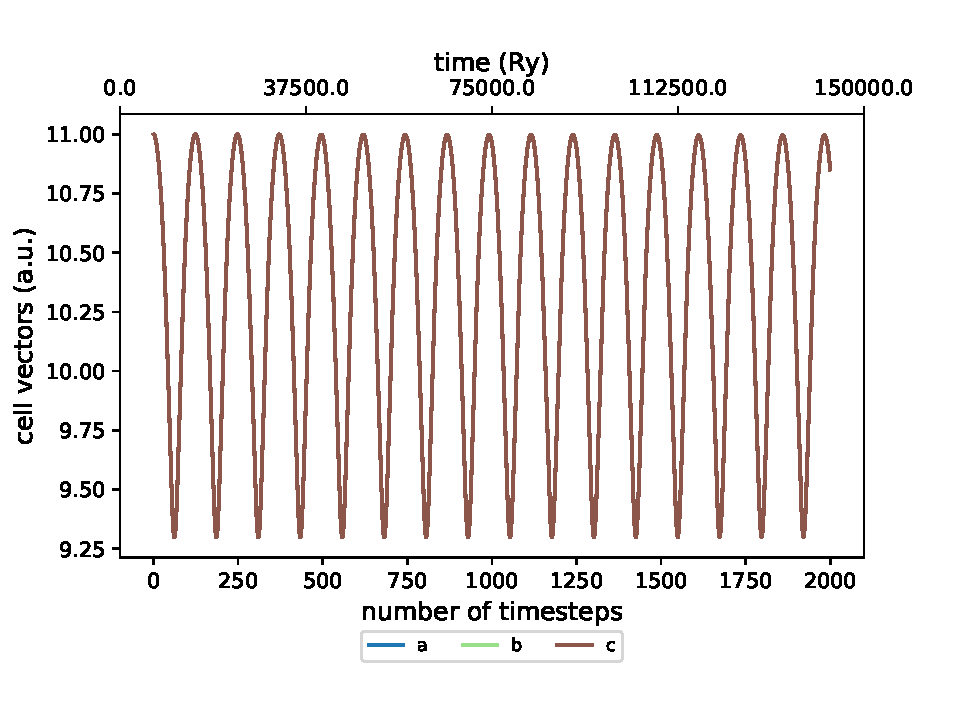
\includegraphics[width=\linewidth]{2000_75_100_2_avec}
		\end{minipage}}
	\caption{Wentzcovitch MD for FCC \ce{Ar} at \SI{0}{\kelvin}, with \texttt{dt}$=75$,
		\texttt{nstep}$=2000$.}
	\label{fig:inp1run}   %% label for entire figure 
\end{figure}

From Fig. \ref{fig:inp1run:mini:subfig:b} we can approximate assume that the stable
lattice parameter is around \SI{9.9}{\bohr}, where vibration happens back and forth.
But the code also provide a \texttt{nm} method by adding a damping to let us compute energy-minimized structure quickly. So we keep the fictitious mass fixed,
and then run the structure minimization algorithm. The stabilized structure also has a
lattice parameter around \SI{9.9}{\bohr}, which strengthen the credibility of our MD result,
see Fig. \ref{fig:inp5} for references.

\begin{figure}[h]
  \subfigure[Energies for structure minimization versus time.]{
    \label{fig:inp5:mini:subfig:a}   %% label for first subfigure 
    \begin{minipage}[b]{0.48\textwidth}
      \centering
      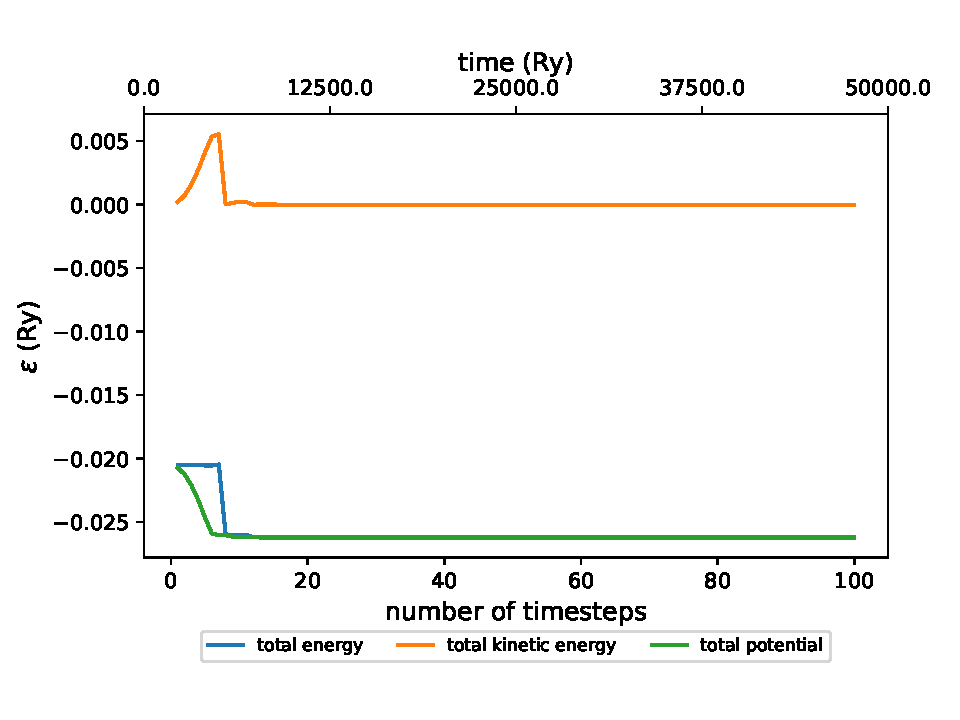
\includegraphics[width=\linewidth]{100_500_2010_9}
  \end{minipage}}
  \hfill
  \subfigure[Lattice parameters for structure minimization versus time, the final result is around \SI{9.9}{\bohr}.]{
    \label{fig:inp5:mini:subfig:b}   %% label for second subfigure 
    \begin{minipage}[b]{0.48\textwidth}
      \centering 
      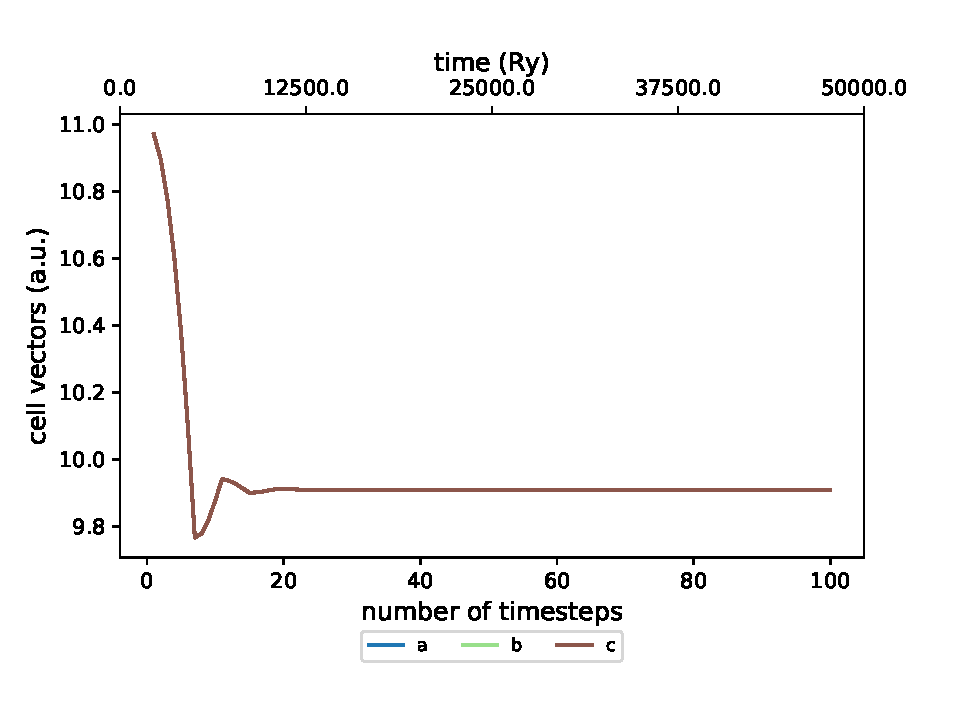
\includegraphics[width=\linewidth]{100_500_2010_3_avec} 
  \end{minipage}}
  \caption{Wentzcovitch's structure minimization algorithm for FCC \ce{Ar}.}
  \label{fig:inp5}   %% label for entire figure 
\end{figure}


First we run the code using Andersen's molecular dynamics, to find the oscillation frequency of atoms. This is done at \SI{0}{\kelvin}, so we have to shift the atoms a little from their equilibrium
positions, or else we will not observe an oscillation frequency, like in Fig. \ref{fig:andersen0:mini:subfig:a}.
For example, in Fig. \ref{fig:andersen0:mini:subfig:b} we can approximately assume that
one period of oscillation is $110$ time steps. We will use this quantity later.
\begin{figure}[h]
	\centering
	\subfigure[Every atom sits in exactly their equilibrium coordinates.]{
		\label{fig:andersen0:mini:subfig:a}   %% label for first subfigure 
		\begin{minipage}[b]{0.48\textwidth}
			\centering
			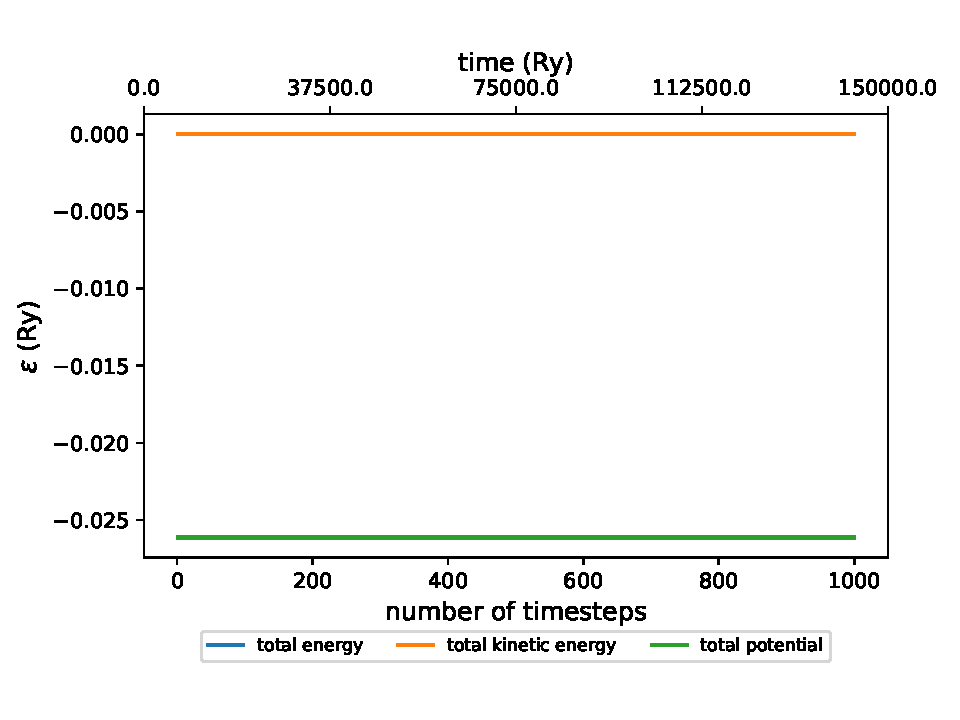
\includegraphics[width=\linewidth]{1000_150_1100_2.pdf}
		\end{minipage}}
	\hfill
	\subfigure[One of the atom shifts a little upon its equilibrium coordinate.]{
		\label{fig:andersen0:mini:subfig:b}   %% label for second subfigure 
		\begin{minipage}[b]{0.48\textwidth}
			\centering
			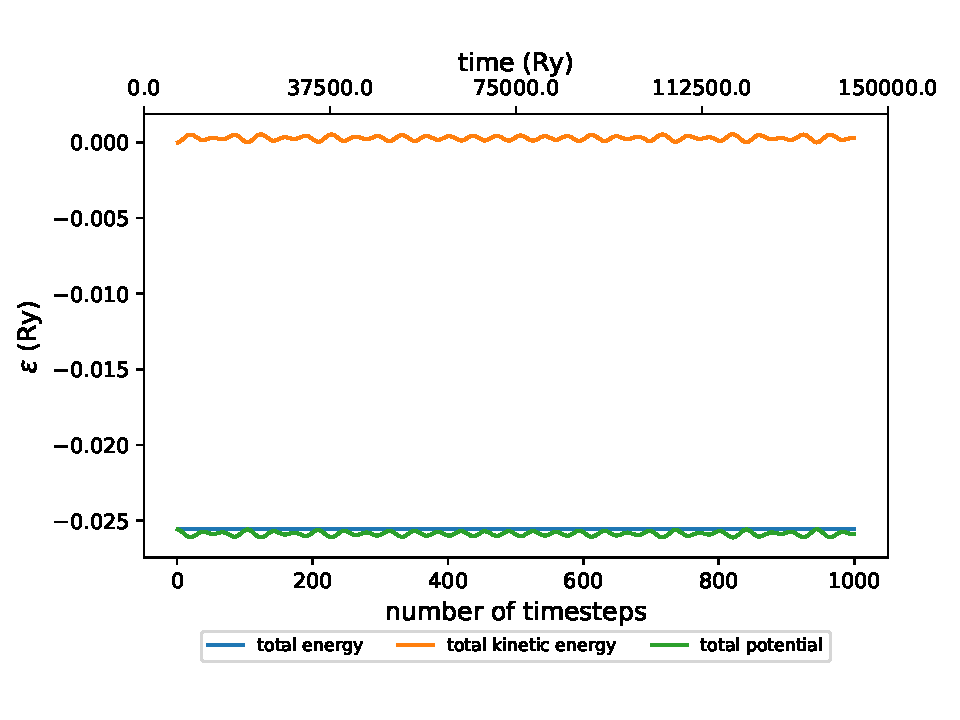
\includegraphics[width=\linewidth]{1000_150_1100-3.pdf}
		\end{minipage}}
	\caption{A conventional FCC cell of \ce{Ar} at \SI{0}{\kelvin}}
	\label{fig:andersen0}   %% label for entire figure 
\end{figure}


%If we keep all other simulation parameters the same, but change
%the size of time steps to $100$ in \texttt{inp2} (\texttt{inp1} is $200$) in Rydberg-like units,
%i.e., decrease step size by a half, the results will be shown in Fig. \ref{fig:input2}.
%There is not much differences from the first results. But looking in detail,
%we can see that the amplitude of atomic potential in Fig. \ref{fig:input2:a} is not decaying
%and the amplitude of lattice kinetic energy in Fig. \ref{fig:input2:l} is also not decaying
%comparing to the corresponding figures Fig. \ref{fig:input1:a} and Fig. \ref{fig:input1:l},
%respectively. And also, the amplitude of lattice parameter is not decaying in
%Fig. \ref{fig:input2:avec} rather than in \ref{fig:input1:avec}. We should also be aware of
%that the oscillation frequency of energies, including kinetic and potential, do not change
%as the time step is decreased to $\frac{ 1 }{ 2 }$, we will discuss later on this phenomenon.
%\begin{figure}[H]
%  \begin{minipage}[t]{0.45\textwidth}
%    \includegraphics[width=\linewidth]{input2/avec_abc}
%    \subcaption{Lattice parameters of \texttt{inp2}.}
%    \label{fig:input2:avec}
%  \end{minipage}
%  \hfil
%  \begin{minipage}[t]{0.45\textwidth}
%    \includegraphics[width=\linewidth]{input2/t}
%    \subcaption{Total energy of \texttt{inp2}.}
%    \label{fig:input2:t}
%  \end{minipage}
%  \hfil
%  \vfill
%  %\vspace*{0.5cm} % (or whatever vertical separation you prefer)
%  \begin{minipage}[t]{0.45\textwidth}
%    \includegraphics[width=\linewidth]{input2/a}
%    \subcaption{Atomic contribution to total energy of \texttt{inp2}.}
%    \label{fig:input2:a}
%  \end{minipage}
%  \hfil
%  \begin{minipage}[t]{0.45\textwidth}
%    \includegraphics[width=\linewidth]{input2/l}
%    \subcaption{Lattice contribution to total energy of \texttt{inp2}.}
%    \label{fig:input2:l}
%  \end{minipage}
%  \caption{Simulation results for \texttt{inp2}.}
%  \label{fig:input2}
%\end{figure}

For \texttt{inp3}, now we shrink the unit cell size to $\frac{ 1 }{ 4 }$ of the
\texttt{inp1}, i.e., there is only $1$ \ce{Ar} atom in the cell. 
Also, the time step is $100$, the same as \texttt{inp2}.
See Fig. \ref{fig:fcc3} for reference.
Now let's see what will happen to the simulation result. 

However, this time, the oscillation frequency of energies and lattice parameters
both increase by a factor of $2$, this is not astonishing because from
\eqref{eq:hdd} we know that
\begin{equation}
	\omega \propto \sqrt{
		\frac{ B }{ W V }
	},
\end{equation}
where $B$ is the bulk modulus.
Here we again see the decaying phenomenon,
comparing to simulation of \texttt{inp1}, we see that the oscillation amplitude of
both
%\begin{figure}[H]
%  \begin{minipage}[t]{0.45\textwidth}
%    \includegraphics[width=\linewidth]{input3/avec_abc}
%    \subcaption{}
%    \label{fig:input3:avec_abc}
%  \end{minipage}
%  \hfil
%  \begin{minipage}[t]{0.45\textwidth}
%    \includegraphics[width=\linewidth]{input3/t}
%    \subcaption{}
%    \label{fig:input3:t}
%  \end{minipage}
%  \hfil
%  \vfill
%  %\vspace*{0.5cm} % (or whatever vertical separation you prefer)
%  \begin{minipage}[t]{0.45\textwidth}
%    \includegraphics[width=\linewidth]{input3/a}
%    \subcaption{}
%    \label{fig:input3:a}
%  \end{minipage}
%  \hfil
%  \begin{minipage}[t]{0.45\textwidth}
%    \includegraphics[width=\linewidth]{input3/l}
%    \subcaption{}
%    \label{fig:input3:l}
%  \end{minipage}
%  \caption{\texttt{inp3}.}
%  \label{fig:input3}
%\end{figure}
